% Research manuscript rewritten around traceable Runalith/AGG empirical artifacts.
% Compile in this directory with: latexmk -xelatex -interaction=nonstopmode -halt-on-error agg_adaptive_goal_graph_research_paper_vi.tex
\documentclass[11pt,a4paper]{article}
\usepackage{fontspec}
\setmainfont{Liberation Serif}
\setsansfont{Liberation Sans}
\setmonofont{DejaVu Sans Mono}[Scale=0.84]
\usepackage[a4paper,margin=2.25cm,headheight=15pt,footskip=20pt]{geometry}
\usepackage{microtype}
\usepackage{amsmath,amssymb}
\usepackage{booktabs,tabularx,longtable,array,multirow}
\usepackage{graphicx}
\usepackage{enumitem}
\setlist{nosep,leftmargin=1.55em}
\usepackage{xcolor}
\definecolor{aggblue}{HTML}{245A8D}
\definecolor{agggray}{HTML}{F2F4F7}
\definecolor{aggmid}{HTML}{526173}
\definecolor{aggorange}{HTML}{D97732}
\usepackage{fancyhdr}
\pagestyle{fancy}
\fancyhf{}
\lhead{\small AGG / Runalith -- nghiên cứu thực nghiệm nội bộ}
\rhead{\small 25-10-2026}
\cfoot{\thepage}
\usepackage{csquotes}
\usepackage[backend=biber,style=ieee,sorting=none,maxbibnames=6,doi=true,isbn=false,url=true,eprint=true]{biblatex}
\addbibresource{agg_adaptive_goal_graph_references.bib}
\usepackage{xurl}
\usepackage[hidelinks,breaklinks=true]{hyperref}
\usepackage[nameinlink,noabbrev]{cleveref}
\usepackage{placeins}
\hypersetup{pdftitle={AGG có mang lại lợi ích đo được không? Đánh giá thực nghiệm theo các giai đoạn phát triển Runalith},pdfauthor={Bản thảo nghiên cứu kỹ thuật nội bộ},pdfsubject={Đánh giá thực nghiệm trên benchmark tổng hợp; chưa qua phản biện độc lập},pdfkeywords={Adaptive Goal Graph, AGG, Runalith, Beam Search, MCTS, benchmark, provenance, knowledge reuse}}
\setlength{\parskip}{0.32em}
\setlength{\parindent}{1.1em}
\setlength{\emergencystretch}{2em}
\renewcommand{\arraystretch}{1.15}
\newcolumntype{Y}{>{\raggedright\arraybackslash}X}
\newcommand{\AGG}{\textsc{Agg}}
\newcommand{\code}[1]{\texttt{\small #1}}
\newcommand{\pp}{\,\text{điểm phần trăm}}
\renewcommand{\tablename}{Bảng}
\renewcommand{\figurename}{Hình}

\title{\vspace{-1.25cm}\color{aggblue}\bfseries AGG có mang lại lợi ích đo được không?\\[0.25em]
\large Đánh giá thực nghiệm theo các giai đoạn phát triển Adaptive Goal Graph trong Runalith}
\author{Bản thảo nghiên cứu kỹ thuật nội bộ\\\normalsize Dữ liệu benchmark từ workspace dự án; chưa qua phản biện độc lập}
\date{25 tháng 10 năm 2026}

\begin{document}
\maketitle
\renewcommand{\abstractname}{Tóm tắt}
\begin{abstract}
Bài báo đánh giá câu hỏi thực nghiệm: trong các giai đoạn phát triển Adaptive Goal Graph (AGG) của Runalith, những lợi ích nào đã được đo lường, lợi ích nào không xuất hiện và đâu là khoảng trống bằng chứng. Các công trình công bố bên ngoài được dùng làm bối cảnh phương pháp, không trộn vào dữ liệu hoặc biểu đồ AGG; nghiên cứu phân tích các ledger benchmark của chính dự án: benchmark thuật toán Phase~1 (28 mẫu tác vụ tổng hợp, 7 cụm tác vụ, 5 seed, 700 lượt chạy trên 5 phương pháp); holdout của discriminator Phase~2 (40 ví dụ tổng hợp); benchmark ghép cặp Phase~2 (5 đồ thị); và benchmark đối kháng Phase~3 (24 đồ thị, 120 lượt ghép cặp). Các số liệu được đối chiếu với artifact nguồn; ledger Phase~1 vượt qua kiểm tra toàn vẹn và khớp hash nguồn hiện tại, còn báo cáo Phase~2 tái tính lại kết quả holdout từ tập đánh giá đã ghim. Kết quả Phase~1 cho thấy AGG Beam width~4 đạt 140/140 kết quả tác vụ đúng, so với 56/140 của width~1 và 105/140 của width~2; width~4 ngang tỷ lệ kết quả đúng quan sát được với tree-search baseline, không vượt trội so với baseline đó. Trong benchmark Phase~2, discriminator đạt 40/40 ví dụ holdout đúng nhưng nhãn là tổng hợp; tìm kiếm ghép cặp vẫn đạt 5/5 ở cả baseline và Phase~2. Trong lớp đồ thị có đường đích của Phase~3, Beam và MCTS cùng đạt 100/100 lượt; MCTS dùng trung bình 11 lần mở rộng và 0,621 ms, so với 5 lần và 0,244 ms của Beam. Trên ca không có đường đích, MCTS không phải thuật toán vét cạn nên không thể xác nhận không có lời giải. Ở Phase~4, ledger ghi nhận một node tri thức xuất hiện xuyên 28 đồ thị mục tiêu, nhưng node chưa được xác minh và chưa đủ điều kiện dùng cho lập kế hoạch; lợi ích về thời gian, chi phí hoặc thành công downstream chưa được đo. Kết luận: AGG có dấu hiệu hữu ích cho chọn đường trong fixture tổng hợp khi dùng beam rộng hơn, nhưng chưa có bằng chứng rằng toàn bộ lộ trình Phase~1--4 cải thiện hiệu quả workflow thực tế hay tổng chi phí end-to-end.
\end{abstract}

\noindent\textbf{Từ khóa:} Adaptive Goal Graph; thực nghiệm phần mềm; Beam Search; discriminator; Monte Carlo Tree Search; provenance; tái sử dụng tri thức.

\section{Giới thiệu và câu hỏi nghiên cứu}

\subsection{Bài toán cần trả lời}
AGG được phát triển nhằm biểu diễn giả thuyết, năng lực, điều kiện, bằng chứng và các phụ thuộc thành đồ thị có thể tìm kiếm; sau đó nối đồ thị đó với workflow runtime và lưu những bài học từ workflow terminal vào kho tri thức. Đề xuất kiến trúc không tự chứng minh giá trị của nó. Giá trị chỉ có thể được xác nhận bằng cách so sánh kết quả và chi phí với một baseline được xác định trước, trên cùng bài toán và cùng điều kiện.

Các nghiên cứu về Tree of Thoughts (ToT), Graph of Thoughts (GoT) và Language Agent Tree Search (LATS) cung cấp các cách tiếp cận liên quan để giữ nhiều ứng viên, mô hình hóa quan hệ giữa các bước, và kết hợp tìm kiếm với hành động/phản hồi \cite{yao2023tot,besta2024got,zhou2024lats}. Chúng là nền tảng khái niệm, không phải baseline định lượng trực tiếp ở đây: benchmark của bài này dùng implementation, workload và oracle khác nhau. Theo chuẩn thực nghiệm phần mềm của ACM SIGSOFT, một đánh giá kỹ thuật cần nêu rõ artifact, workload, metric, phép đo, khả năng tái lập và phạm vi khái quát hóa; những điều kiện này đặc biệt quan trọng khi dữ liệu chỉ là tổng hợp \cite{acmsigsoftstandards}.

Bài báo sử dụng bốn câu hỏi nghiên cứu (RQ):
\begin{description}[style=nextline,leftmargin=1.7em]
\item[RQ1 -- Tìm kiếm Phase~1.] Beam width rộng hơn có tăng tỷ lệ kết quả đúng không, và chi phí tính toán tăng bao nhiêu?
\item[RQ2 -- Discriminator Phase~2.] Có bằng chứng độc lập trên holdout tổng hợp cho bộ phân biệt không, và nó có cải thiện kết quả tìm kiếm trong phép so sánh ghép cặp không?
\item[RQ3 -- MCTS Phase~3.] MCTS có tăng khả năng tìm đường đích hoặc giảm chi phí so với Beam không? Khả năng tìm đường có được tách khỏi khả năng chứng minh không tồn tại đường đi không?
\item[RQ4 -- Reuse Phase~4 và giá trị tổng thể.] Tri thức được capture đã được xác minh và sử dụng để cải thiện workflow sau đó chưa? Các kết quả theo giai đoạn có chứng minh lợi ích end-to-end không?
\end{description}

Một \emph{lợi ích đo được} trong nghiên cứu này là thay đổi về metric kết quả (tỷ lệ tác vụ đúng, đường đi hợp lệ, phân loại holdout) hoặc metric chi phí (số cạnh mở rộng, thời gian, token) dưới một phép so sánh được mô tả rõ. Một thay đổi kiến trúc, số test pass hoặc bản ghi được lưu thành công không được xem là lợi ích người dùng trừ khi nó gắn với outcome tương ứng.

\section{Thiết kế nghiên cứu và nguồn dữ liệu}

\subsection{Thiết kế}
Đây là nghiên cứu đánh giá kỹ thuật dựa trên các artifact benchmark đã lưu của workspace Runalith/AGG, kết hợp phân tích định lượng và kiểm tra provenance. Các giá trị trong hình và bảng được lấy từ summary/per-case rows của các artifact xác định, không suy ra từ biểu đồ văn liệu và không được tạo ngẫu nhiên cho bài báo. Nghiên cứu không thực hiện lại benchmark production, không có nhóm người dùng và không có thử nghiệm A/B end-to-end trên workflow thật.

Cách trình bày tuân theo các nguyên tắc thiết yếu của ACM SIGSOFT Empirical Standards: câu hỏi rõ ràng; phương pháp và cách lấy dữ liệu được mô tả; metric được định nghĩa; kết quả gắn với câu hỏi; và giới hạn được nêu cạnh diễn giải \,\cite{acmsigsoftstandards}. Các kết quả công khai từ tài liệu nền tảng không được chép thành biểu đồ AGG hoặc trộn vào mẫu số nội bộ.

\subsection{Bộ dữ liệu và artifact được phân tích}
Bảng~\ref{tab:datasets} tổng hợp các nguồn dữ liệu được dùng cho từng câu hỏi. Các bộ đánh giá được phân tích riêng theo vai trò; không gộp các mẫu số khác nhau thành một điểm hiệu quả chung.
\begin{table}[htbp]
\centering\small
\begin{tabularx}{\linewidth}{p{2.2cm} p{3.15cm} p{2.05cm} Y}
\toprule
\textbf{Giai đoạn} & \textbf{Artifact / dữ liệu} & \textbf{Quy mô} & \textbf{Chất lượng bằng chứng / vai trò trong kết luận}\\
\midrule
Phase~1 & Ledger thuật toán trên catalog tổng hợp đã đóng băng & 28 template; 7 cụm; 140 graph-instance; 700 trial & Bộ phân tích chính. Ledger được xác minh toàn vẹn; các hash nguồn trong ledger khớp source hiện tại. Vẫn là dữ liệu synthetic, không phải holdout production.\\
Phase~2-A & Holdout discriminator trên dataset tổng hợp & 40 ví dụ; 20 positive, 20 negative & Báo cáo đánh giá đã tái tính metric từ split holdout; nhãn chưa được adjudication độc lập. Dùng để đánh giá classifier, không phải success rate workflow.\\
Phase~2-B & Paired search benchmark & 5 đồ thị ghép cặp & Cả baseline và Phase~2 đều đúng 5/5; quá nhỏ để xác nhận khác biệt latency.\\
Phase~3 & Adversarial synthetic graph corpus & 24 đồ thị; 5 seed; 120 trial ghép cặp & Dùng để tách goal-path discovery khỏi no-solution proof. Chỉ là offline shadow/synthetic replay; chưa có acceptance vận hành.\\
Phase~4 & Trường reuse trong ledger Phase~1 và mô tả luồng capture & 28 goal graphs; 1 distinct reused node & Có dấu vết membership, nhưng node chưa xác minh và chưa usable for planning; không có đo lường tiết kiệm.\\
\bottomrule
\end{tabularx}
\caption{Tổng quan nguồn bằng chứng. Quy mô trial không đồng nghĩa số tác vụ độc lập; các trial dùng lại cùng tập template/nhóm tác vụ.}
\label{tab:datasets}
\end{table}

\subsection{Metric và cách tính}
\begin{itemize}
\item \textbf{Task-outcome accuracy:} phần lượt mà phương pháp đưa ra đúng kết quả của oracle độc lập với thuật toán tìm kiếm. Với đồ thị có lời giải, phải trả về đường đi hợp lệ có đủ điều kiện/phụ thuộc; với đồ thị vô nghiệm, chỉ câu trả lời “không có đường” sau khi tìm kiếm kết thúc đầy đủ mới được tính đúng.
\item \textbf{Goal-path success:} chỉ tính các đồ thị có ít nhất một đường đi hợp lệ; không gộp với bài toán chứng minh vô nghiệm.
\item \textbf{Expansion count:} số successor-edge examinations trong bộ đếm tìm kiếm. Đây không phải toàn bộ computation; ToT thực hiện tiền xử lý khoảng cách toàn đồ thị, được báo cáo riêng.
\item \textbf{Runtime:} thời gian thực thi phương pháp đồng bộ đo bằng đồng hồ monotonic; có thể dao động theo host. Không diễn giải millisecond từ benchmark nhỏ thành latency của workflow end-to-end.
\item \textbf{Classifier holdout metrics:} accuracy, balanced accuracy, precision, recall, F1, log loss và Brier score; khoảng tin cậy Wilson 95\% được giữ như báo cáo đánh giá đã lưu \,\cite{newcombe1998wilson}.
\item \textbf{Knowledge reuse:} số node có identity xuyên nhiều goal graph, số node được xác minh và số node đã được cấp điều kiện dùng để lập kế hoạch. Không suy ra tiết kiệm từ membership đơn thuần.
\end{itemize}

\subsection{Bất định, ghép cặp và tính toàn vẹn}
Phase~1 có năm repeat seed trên 28 template, nhưng chỉ bảy cụm family độc lập ở mức thiết kế. Với phép so sánh Beam width~1 với width~4, khoảng tin cậy percentile bootstrap 95\% được lấy bằng cách resample bảy cụm family và giữ nguyên các quan sát ghép cặp trong mỗi cụm; 10.000 lần lặp. Khoảng này là mô tả sự nhạy cảm của kết quả trên phân phối cụm synthetic, không phải kiểm định xác nhận trên tổng thể workflow. Wilson CI của Phase~2 holdout là CI nhị thức trên 40 ví dụ; giả định độc lập giữa nhãn không được xác lập qua một nghiên cứu thực địa.

Trạng thái được đánh giá riêng theo từng artifact. Ledger Phase~1 vượt qua kiểm tra toàn vẹn và khớp hash nguồn hiện tại, nhưng điều đó không đồng nghĩa với chấp nhận vận hành. Báo cáo Phase~2 tái tính lại metric holdout và benchmark ghép cặp; dữ liệu vẫn là tổng hợp và chưa được chấp nhận làm bằng chứng vận hành. Phase~3 chỉ là replay tổng hợp ở chế độ shadow. Một pilot local-LLM lịch sử bị loại khỏi phân tích định lượng chính vì hash runtime trong ledger không khớp source hiện tại và phép so sánh không cùng điều kiện với thuật toán tìm kiếm xác định.

\section{Kết quả Phase 1: Beam width làm tăng độ đúng, nhưng có chi phí}

\subsection{Tỷ lệ kết quả đúng}
Hình~\ref{fig:phase1accuracy} thể hiện kết quả từ 700 lượt chạy, 140 trial cho mỗi phương pháp. Catalog có 21 template có lời giải và 7 template vô nghiệm; mỗi template được tạo lại dưới năm seed. Vì vậy, tỷ lệ là thống kê mô tả trên fixture, không phải ước lượng đại diện cho 140 tác vụ production độc lập.

\begin{figure}[htbp]
\centering
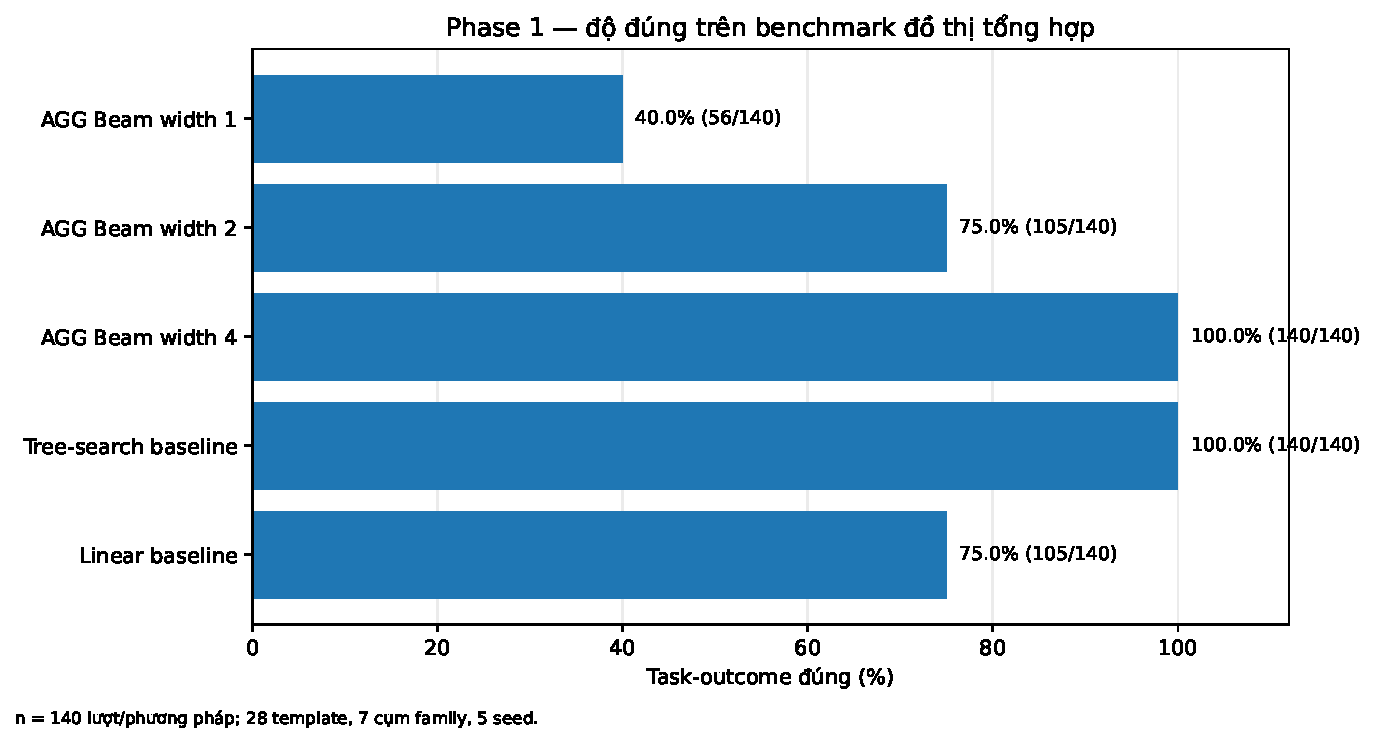
\includegraphics[width=0.95\linewidth]{fig1_phase1_outcome_accuracy.pdf}
\caption{Tỷ lệ task-outcome đúng trong benchmark Phase~1 của chính AGG. Mỗi cột là 140 lượt chạy; số trên cột là lượt đúng/tổng lượt. Width~4 đạt 100\% trong catalog đã đóng băng, ngang tree-search baseline trên metric này.}
\label{fig:phase1accuracy}
\end{figure}

\begin{table}[htbp]
\centering\small
\setlength{\tabcolsep}{5pt}
\begin{tabularx}{\linewidth}{p{2.7cm} p{2.8cm} p{3.0cm} Y}
\toprule
\textbf{Phương pháp} & \shortstack{\textbf{Outcome đúng}\\\textbf{(n/140)}} & \shortstack{\textbf{Số lần mở rộng}\\\textbf{trung bình}} & \shortstack{\textbf{Thời gian trung bình / P95}\\\textbf{(ms)}}\\
\midrule
AGG Beam $w=1$ & 40,0\% (56/140) & 7,31 & 0,814 / 1,326\\
AGG Beam $w=2$ & 75,0\% (105/140) & 10,87 & 1,066 / 2,191\\
AGG Beam $w=4$ & 100\% (140/140) & 12,46 & 1,194 / 2,001\\
Tree-search baseline & 100\% (140/140) & 10,93 & 0,101 / 0,193\\
Linear baseline & 75,0\% (105/140) & 16,32 & 0,057 / 0,102\\
\bottomrule
\end{tabularx}
\caption{Tóm tắt benchmark Phase~1. Accuracy bao gồm cả đồ thị có lời giải và đồ thị vô nghiệm. Beam~2 đạt 100\% trên ca có đường đích nhưng 0\% ở ca vô nghiệm; Beam~4 và tree-search baseline đạt 100\% ở cả hai lớp. Thời gian là số đo trên host của benchmark.}
\label{tab:phase1results}
\end{table}

Tăng width từ 1 lên 2 nâng task-outcome accuracy 35 điểm phần trăm; từ 2 lên 4 tăng thêm 25 điểm; tổng mức tăng width~1 lên width~4 là 60 điểm phần trăm. So sánh ghép cặp width~4 trừ width~1 cho chênh lệch 0,60; CI bootstrap theo bảy cụm family là [0,371; 0,893]. Đây là khoảng mô tả theo các cụm synthetic đang có; số cụm nhỏ nên không nên coi là bằng chứng xác nhận về năng lực tổng quát.

Một chi tiết quan trọng là beam width~2 tìm đường đúng trên toàn bộ 105/105 lượt có lời giải nhưng nhận sai ở toàn bộ 35/35 lượt vô nghiệm vì không có bằng chứng kết thúc vét cạn. Vì vậy, overall outcome accuracy của Beam~2 chỉ là 75\%.

\subsection{Chi phí tìm kiếm}
\begin{figure}[htbp]
\centering
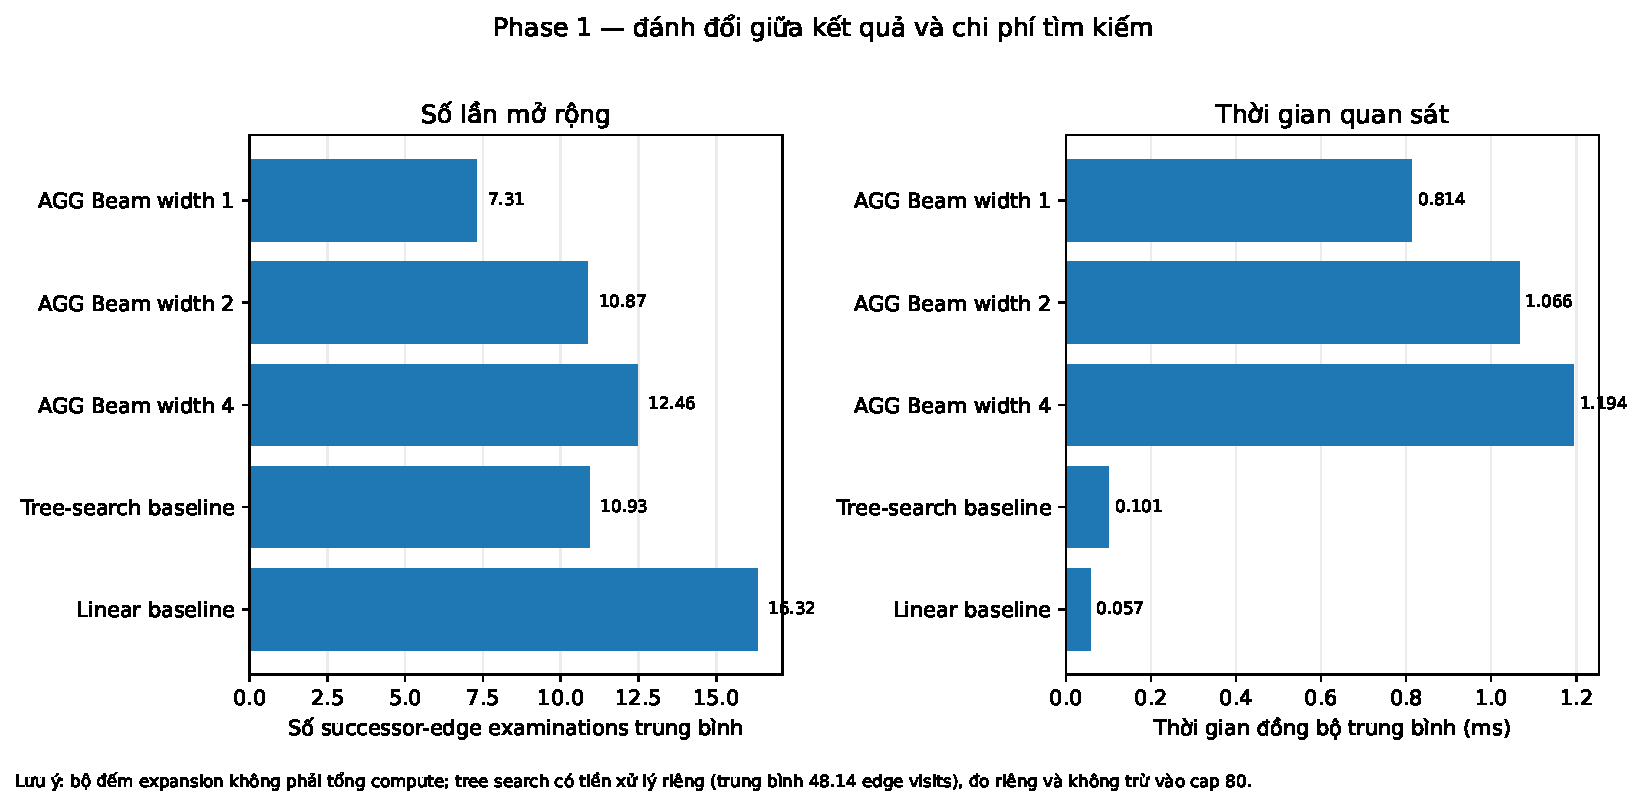
\includegraphics[width=0.98\linewidth]{fig2_phase1_cost_tradeoff.pdf}
\caption{Thời gian đồng bộ và bộ đếm successor-expansion trung bình theo phương pháp. Hai panel giữ đơn vị tách biệt. Tree search còn có tiền xử lý khoảng cách ngược toàn đồ thị, trung bình 48,14 lần kiểm tra cạnh; số đó được đo riêng và không trừ vào giới hạn 80 successor expansions.}
\label{fig:phase1cost}
\end{figure}

Beam~4 tiêu tốn nhiều expansions hơn Beam~1 khoảng 70,6\%, và thời gian trung bình cao hơn 46,8\%. So với Beam~2, thời gian cao hơn khoảng 12,0\%. Đây là một đánh đổi hữu hình: beam rộng hơn hữu ích khi tiêu chí là đúng kết quả trong fixture này, nhưng không miễn phí.

Tree-search baseline cũng đạt 140/140 kết quả đúng và có mean runtime 0,101 ms trong lần benchmark này, thấp hơn thời gian đo của Beam~4 (1,194 ms). Không nên kết luận AGG có lợi thế tốc độ so với tree search trên các số liệu này. Mặt khác, ngân sách 80 là giới hạn bộ đếm successor-expansion chứ không phải giới hạn tổng computation đồng nhất; Tree search có phần tiền xử lý riêng, trong khi các phương pháp khác có các chi phí lọc/lookahead riêng. Do đó, kết quả hiện tại hỗ trợ một kết luận hẹp về hiệu quả Beam width trên catalog, không đủ để xếp hạng tổng quát hiệu quả của các thuật toán.

\section{Kết quả Phase 2: classifier tốt trên synthetic holdout, nhưng lợi ích tìm kiếm chưa được xác nhận}

\subsection{Đánh giá discriminator trên holdout}
Bộ dữ liệu discriminator có 20 ví dụ positive và 20 negative trong holdout. Báo cáo đánh giá ghi nhận accuracy, balanced accuracy, precision, recall và F1 đều bằng 100\%; confusion matrix không có false positive hoặc false negative. Log loss là 0,0119 và Brier score là 0,000153. Wilson CI 95\% cho accuracy là 91,24--100\%.

\begin{figure}[htbp]
\centering
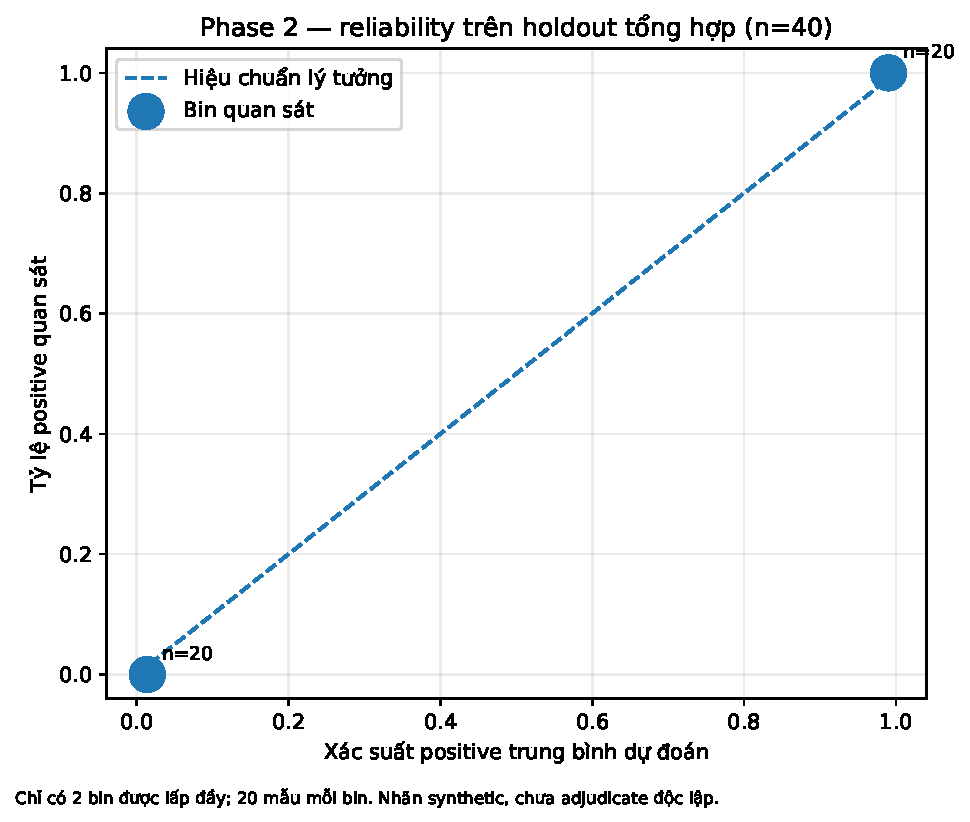
\includegraphics[width=0.82\linewidth]{fig3_phase2_reliability.pdf}
\caption{Reliability diagram của discriminator Phase~2 trên 40 ví dụ holdout tổng hợp. Chỉ hai bin có quan sát: 20 dự đoán negative với xác suất positive trung bình 0,0139 và 20 positive với xác suất trung bình 0,9903. Các metric phân loại hoàn hảo trên một tập tổng hợp không chứng minh classifier đã hiệu chuẩn hoặc tổng quát hóa trên dữ liệu thật.}
\label{fig:phase2calibration}
\end{figure}

Kết quả này cho thấy mô hình phân biệt học được ranh giới rõ ràng trên split được dùng để đánh giá. Nó không chứng minh rằng nhãn phản ánh workflow thực tế: dataset được xác định là synthetic, chưa có adjudication độc lập hoặc chữ ký xác nhận nhãn. Accuracy là metric của classifier trên 40 dòng; không đồng nhất với tỷ lệ workflow thành công.

\subsection{Tìm kiếm ghép cặp Phase 2}
Trong benchmark năm đồ thị, baseline và Phase~2 đều đưa ra kết quả đúng ở 5/5 ca; mean expansion count cùng bằng 4. Thời gian trung bình đo được giảm từ 1,273 ms xuống 0,690 ms ở lần chạy này, giảm quan sát được khoảng 45,8\%.

\begin{figure}[htbp]
\centering
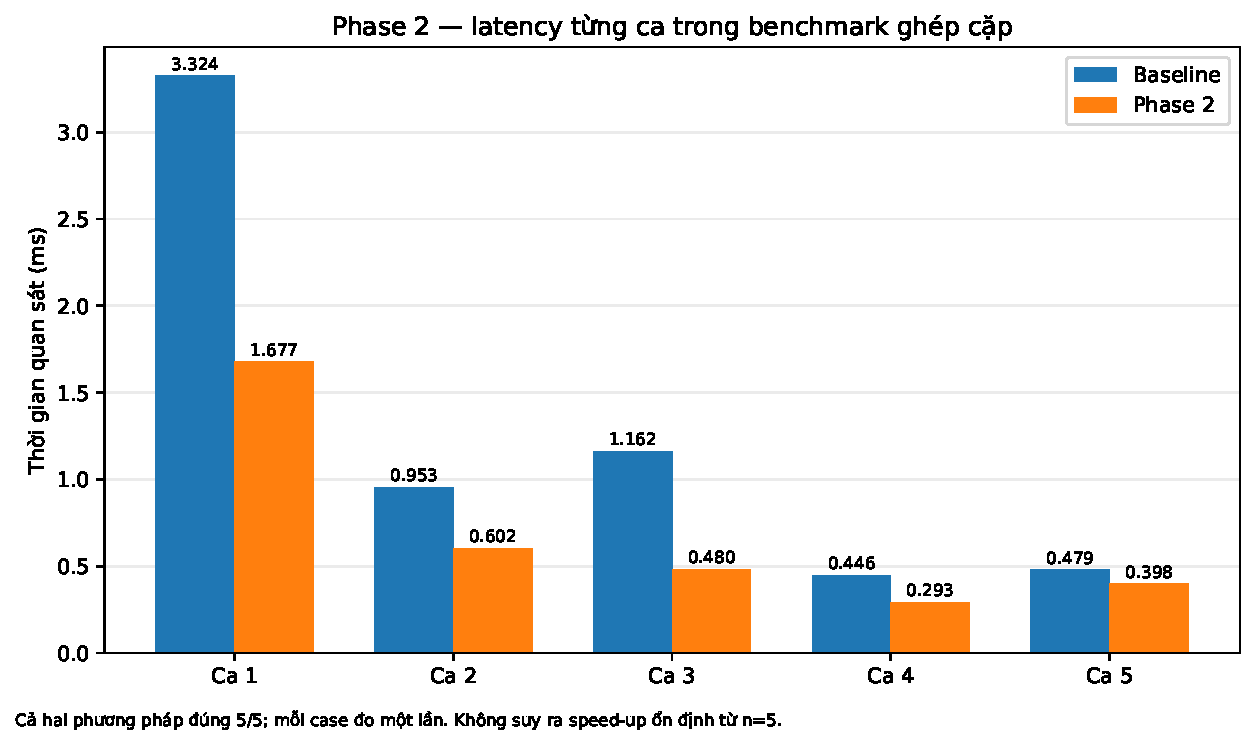
\includegraphics[width=0.86\linewidth]{fig4_phase2_paired_latency.pdf}
\caption{Runtime từng ca của phép so sánh ghép cặp Phase~2. Tất cả năm ca đều đúng với cả hai phương pháp; đồ thị chỉ mô tả số đo trong một lần chạy cho mỗi ca. Không có lặp độc lập đủ để kết luận giảm latency ổn định.}
\label{fig:phase2latency}
\end{figure}

Vì $n=5$, không có ước lượng CI hợp lệ được báo cáo cho chênh lệch paired runtime; những số millisecond nhỏ này nhạy với lịch chạy và overhead. Kết luận cho RQ2 là: holdout classifier có metric tốt trên synthetic data, nhưng paired search benchmark chưa cho thấy cải thiện độ đúng, và tốc độ mới chỉ là tín hiệu quan sát cần benchmark lặp lại trên corpus lớn hơn.

\section{Kết quả Phase 3: MCTS không cải thiện goal-path success trong corpus này}

Benchmark Phase~3 dùng 24 đồ thị tổng hợp độc nhất: 20 đồ thị có đường đích và 4 đồ thị không có đường đích; với năm seed tạo 120 trial ghép cặp. Báo cáo benchmark phân biệt rõ \emph{tìm đường đích} và \emph{chứng minh không có đường đi}, bởi MCTS được triển khai ở chế độ không vét cạn.

\begin{figure}[htbp]
\centering
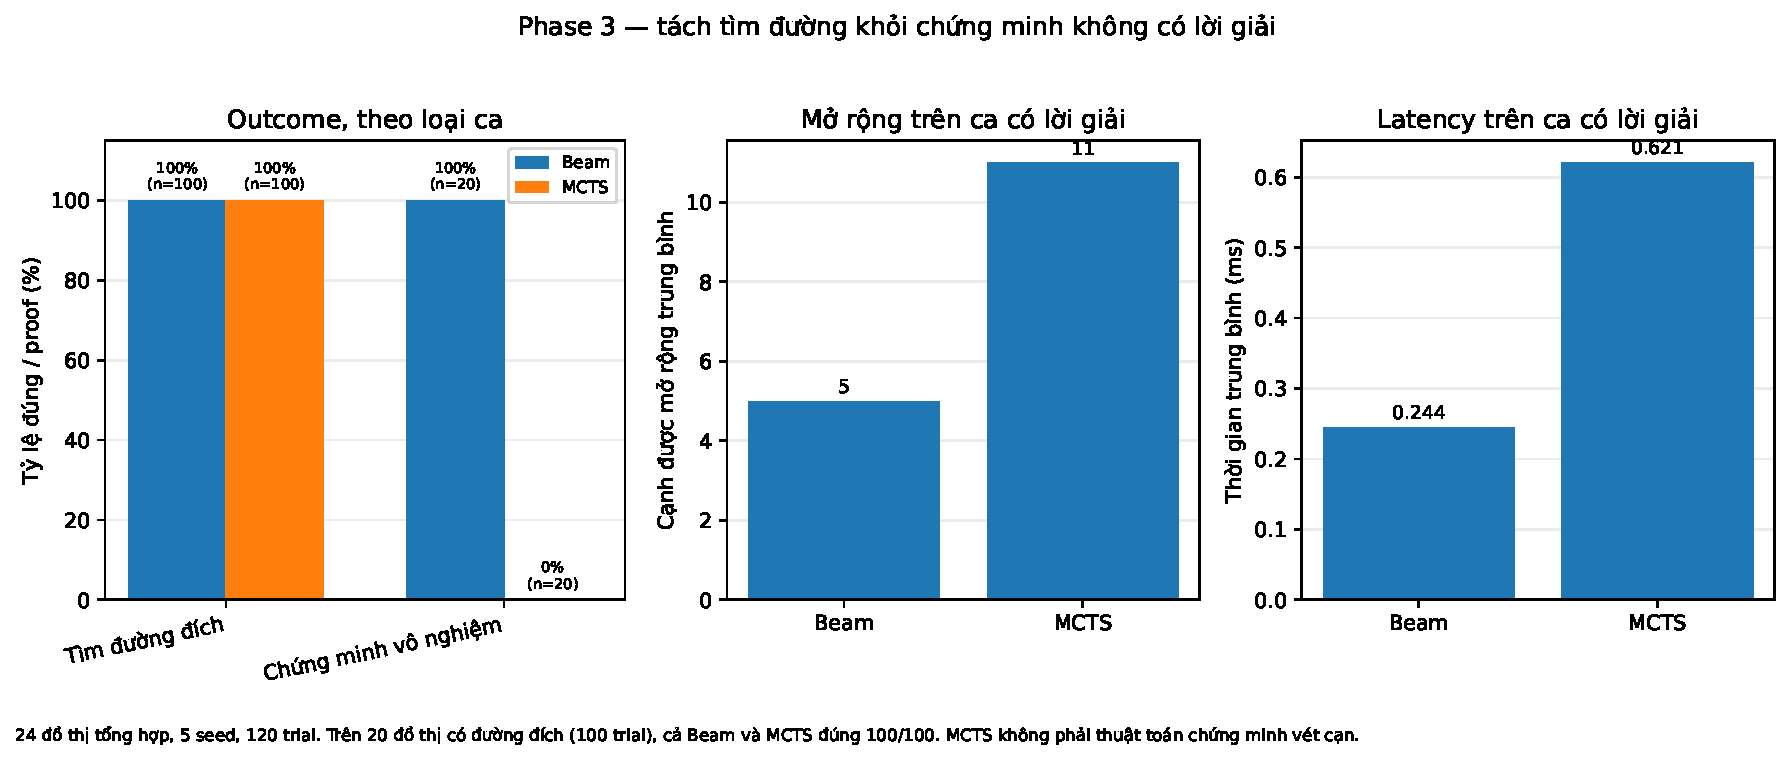
\includegraphics[width=0.98\linewidth]{fig5_phase3_beam_mcts.pdf}
\caption{So sánh Phase~3 theo loại tác vụ, không gộp hai năng lực khác nhau. Goal-path subset: Beam và MCTS đều đúng 100/100 trial. No-solution subset: Beam chứng minh hết 20/20 trial; MCTS 0/20 vì không được định nghĩa là thuật toán chứng minh vét cạn. Panel chi phí chỉ dùng các graph có đường đích.}
\label{fig:phase3}
\end{figure}

Trên tập goal-path, cả hai phương pháp đều đạt 100/100 lượt đúng; chênh lệch success rate bằng 0 điểm phần trăm. Tuy nhiên, MCTS dùng trung bình 11 successor expansions và 0,621 ms/trial, so với 5 expansions và 0,244 ms của Beam. Tỷ số runtime quan sát được là khoảng 2,54 lần; expansion count cao hơn 120\%. MCTS còn dùng 64 simulations và trung bình 943,2 work units theo định nghĩa của benchmark.

Trên bốn ca vô nghiệm, Beam chứng minh không có đường đi bằng tìm kiếm vét cạn ở 20/20 trial. MCTS không có hợp đồng chứng minh no-solution, vì vậy 0/20 là giới hạn capability theo thiết kế, không phải bằng chứng rằng nó tìm đường sai trong các ca có đường. Kết luận cho RQ3: với corpus này, chưa có lợi ích đo được về goal-path success từ MCTS; chi phí tìm kiếm cao hơn và khả năng proof no-solution thấp hơn do không vét cạn. MCTS vẫn có thể đáng nghiên cứu cho không gian trạng thái lớn, nhưng dữ liệu hiện tại không biện minh cho việc nó cải thiện AGG ở fixture này.

\section{Kết quả Phase 4: đã có dấu vết reuse, chưa có lợi ích downstream}

Ledger Phase~1 có trường reuse ghi nhận 28 goal graph và một định danh node được dùng xuyên các goal. Tuy nhiên, node đó có trạng thái \code{verified=false} và \code{usableForPlanning=false}. Không có số đo về thời gian làm workflow, token, số lần làm lại, success rate sau khi reuse, hoặc chi phí được giảm nhờ knowledge capture.

\begin{figure}[htbp]
\centering
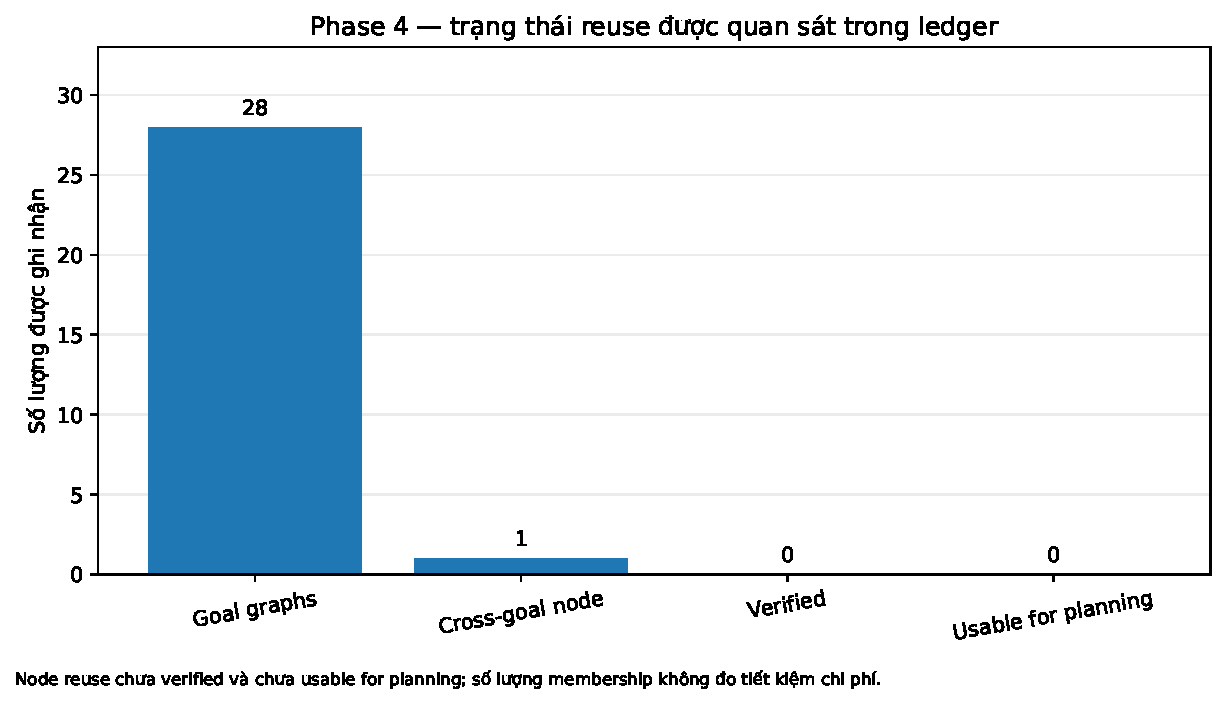
\includegraphics[width=0.9\linewidth]{fig6_phase4_reuse_status.pdf}
\caption{Trạng thái reuse có thể truy nguyên. Một node có membership xuyên nhiều goal graph; không có node nào trong dữ liệu quan sát vừa được xác minh vừa đủ điều kiện dùng cho lập kế hoạch. Đây không phải số đo tỷ lệ tiết kiệm.}
\label{fig:phase4reuse}
\end{figure}

Sự tồn tại của record bền vững là một kết quả triển khai, không phải kết quả hiệu quả. Để chứng minh Phase~4 có ích, cần một thí nghiệm prospective: xác định trước các mục tiêu lặp lại; đo thời gian/tokens/công sửa khi planner không dùng và có dùng tri thức được capture; chỉ bật reuse sau khi lesson được review/verify; tính cả trường hợp reuse gây sai lệch hoặc dùng nhầm provenance. Tới lúc đó, RQ4 chỉ có thể trả lời là \emph{cơ chế capture/reuse có dấu vết cấu trúc, nhưng tác động đến hiệu quả workflow chưa đo được}.

\section{So sánh xuyên các giai đoạn và câu trả lời tổng hợp}

\begin{table}[htbp]
\centering\small
\begin{tabularx}{\linewidth}{p{1.4cm} p{3.35cm} p{3.0cm} Y}
\toprule
\textbf{Giai đoạn} & \textbf{Kết quả định lượng trực tiếp} & \textbf{Lợi ích quan sát được} & \textbf{Điều chưa được chứng minh}\\
\midrule
Phase~1 & Beam~1: 40\%; Beam~2: 75\%; Beam~4: 100\%; tree-search: 100\% task-outcome accuracy trên 140 trial/method & Beam rộng hơn xử lý được nhiều kết quả đúng hơn trong fixture; +60 điểm phần trăm từ width~1 đến width~4 & Không chứng minh ưu thế so với tree-search baseline; Beam rộng hơn tốn nhiều expansions và runtime.\\
Phase~2 & Discriminator: 40/40 đúng trên holdout tổng hợp; paired search: 5/5 so với 5/5 & Có phân tách classifier tốt trên dữ liệu tổng hợp; runtime quan sát thấp hơn ở phép thử 5 ca & Không có tăng accuracy tìm kiếm trong paired benchmark; chưa chứng minh nhãn đại diện hoặc speed-up ổn định.\\
Phase~3 & Goal paths: Beam 100/100, MCTS 100/100; MCTS 11 expansions / 0,621 ms so với Beam 5 / 0,244 ms & Không thấy tăng goal-path success trong corpus đã đo & MCTS tốn nhiều compute hơn và không chứng minh no-solution; lợi ích thích nghi chưa được xác nhận.\\
Phase~4 & Một node reuse xuyên 28 goal graphs; chưa verified và chưa usable for planning & Có định danh reuse để theo dõi bằng dữ liệu & Chưa đo giảm thời gian, chi phí hay tăng success nhờ reuse.\\
\bottomrule
\end{tabularx}
\caption{Bằng chứng theo giai đoạn. Các dòng không có cùng đơn vị đánh giá, vì vậy bảng không phải xếp hạng trực tiếp giữa các phase.}
\label{tab:phasesynthesis}
\end{table}

Câu trả lời cho câu hỏi trung tâm cần chia làm hai mức:
\begin{enumerate}
\item \textbf{Trong các benchmark kỹ thuật tổng hợp: có một số lợi ích cụ thể.} Beam width là yếu tố tạo cải thiện độ đúng lớn nhất trong Phase~1. Phase~2 cho thấy classifier có thể tách lớp tốt trên holdout tổng hợp; Phase~4 có dấu vết lưu identity tri thức xuyên goal graph.
\item \textbf{Trong phát triển end-to-end của AGG: chưa đủ bằng chứng để nói các phase cộng dồn thành lợi ích thực tế.} Phase~2 chưa làm tăng độ đúng tìm kiếm trong paired sample 5 ca; Phase~3 không cải thiện goal-path success và tăng chi phí; Phase~4 chưa đưa node reuse vào trạng thái có thể dùng an toàn hoặc đo được lợi ích. Chưa có thí nghiệm A/B qua các workflow vận hành thật để đo success, retry, thời gian hoàn thành, chi phí công cụ/model và lỗi an toàn.
\end{enumerate}

Một benchmark operational có ý nghĩa cần so sánh plugin/AGG-enabled với basic-tools hoặc baseline hiện hành trên cùng input, permission, môi trường và acceptance criteria. Tài liệu protocol nội bộ xác định mười scenario vận hành và rubric 100 điểm; các benchmark thuật toán synthetic trong bài này không thay thế phép so sánh đó. Trạng thái readiness `BLOCKED`, execution gate \code{CLOSED} và \code{PARTIAL\_NOT\_ACCEPTED} phải được giữ riêng với điểm số offline: đạt điểm benchmark không tự động tạo quyền thực thi hoặc chấp nhận phát hành.

\section{Thảo luận}

\subsection{Lợi ích chính hiện tại là bounded search, không phải memory reuse}
Dữ liệu trực tiếp mạnh nhất là độ nhạy với beam width. Width~1 bỏ lỡ nhiều tuyến và không chứng minh được các đồ thị vô nghiệm; width~4 giữ đủ lựa chọn trong catalog này và đạt outcome đúng. Nhưng tree-search baseline cũng đạt outcome đúng 100\%, với thời gian đo thấp hơn trong bản benchmark này. Vì vậy, một tuyên bố đúng là “beam width có tác động lớn tới chất lượng trên fixture” chứ không phải “AGG tốt hơn các phương pháp search đã biết”.

\subsection{Classifier hoàn hảo trên synthetic holdout không đồng nghĩa generalization}
Các chỉ số Phase~2 gần như hoàn hảo nhưng chính nguồn dữ liệu khai báo corpus synthetic và chưa được xác nhận nhãn độc lập. Khi nhãn tạo theo bộ quy tắc tương tự feature space, một classifier có thể học được bộ quy tắc đó mà không giải quyết các trường hợp mơ hồ, thiếu provenance hoặc thay đổi phân phối trong tác vụ thật. Do đó, holdout chỉ là kiểm tra kỹ thuật nội bộ, không phải đánh giá giá trị sử dụng.

\subsection{MCTS cần justification theo outcome và resource}
MCTS là phương pháp hợp lý khi exploration/exploitation cần thiết trong cây tìm kiếm lớn \,\cite{kocsis2006uct}. Nhưng trong corpus hiện tại, Beam đã đạt 100\% goal-path discovery; MCTS làm tăng expansion count và latency, trong khi vẫn không chứng minh được không có lời giải. Hợp lý nhất là hoãn khẳng định “MCTS tăng hiệu quả” đến khi có corpus có branching/depth thực tế, ngân sách tổng computation tương đương, và một outcome mà MCTS có thể cải thiện thật sự.

\subsection{Provenance là điều kiện quản trị, không phải metric hiệu suất}
Một record gắn source, job và revision giúp truy nguyên, nhưng không chứng minh lesson đúng. W3C PROV-O phân biệt entity, activity và agent; khung quản trị rủi ro AI của NIST nhấn mạnh đánh giá, đo lường, quản lý rủi ro và trách nhiệm xuyên vòng đời \,\cite{w3cprovo,nistairmf2023,nistgenai2024}. Tương tự, lưu knowledge không nên tự động cấp quyền để knowledge đó điều khiển planner hoặc runtime. Đây là lý do trạng thái verified và usable-for-planning phải tách biệt.

\section{Giới hạn và nguy cơ diễn giải sai}
\begin{itemize}
\item \textbf{Tính đại diện:} dữ liệu Phase~1 và Phase~3 là đồ thị tổng hợp. Phase~1 chỉ có bảy cụm family; nhiều trial là bản dựng lại của một số ít template. Không thể khái quát trực tiếp ra nhiệm vụ production.
\item \textbf{Không có đối chứng end-to-end:} bài không đo toàn bộ chu kỳ từ yêu cầu người dùng đến workflow terminal, bao gồm tool use, retries, human review, model tokens và thiệt hại khi sai. Runtime của hàm tìm kiếm không phải runtime của agent.
\item \textbf{Ngân sách tìm kiếm:} cap 80 ở Phase~1 chỉ áp cho counter successor expansions. Chi phí tiền xử lý và các thao tác phụ khác không được chuẩn hóa thành một total-compute budget giống hệt nhau.
\item \textbf{Timing:} runtime là quan sát host-dependent. Phase~2 chỉ có năm cặp và không có repeated timing per case; chênh lệch không nên được gọi là tốc độ cải thiện bền vững.
\item \textbf{Nhãn và oracle:} các oracle kiểm tra tính nhất quán với corpus synthetic, không được adjudicate độc lập trên nhiệm vụ thực. Classifier holdout có số lỗi bằng không nhưng vẫn có bất định và nguy cơ lệch phân phối.
\item \textbf{Local LLM pilot lịch sử:} số liệu trong phụ lục không dùng cho kết luận chính bởi ledger verifier báo hash graph-runtime không khớp source hiện tại; cấu hình cũng chỉ là một-shot prompt ToT-style chứ không phải ToT đa vòng đầy đủ.
\item \textbf{Reuse:} số membership không phải số lần tiết kiệm công việc. Chưa có thử nghiệm tắt/bật reuse hoặc đo hiệu quả quyết định sau reuse.
\item \textbf{Acceptance và trust:} xác minh hash là kiểm tra identity/integrity của byte theo manifest; nó không chứng minh chủ thể, tính đúng của claim, sự đồng thuận của owner hay acceptance production.
\end{itemize}

\section{Thiết kế thí nghiệm tiếp theo để xác nhận lợi ích}
Một nghiên cứu xác nhận nên đăng ký trước bốn nhóm outcome:
\begin{enumerate}
\item \textbf{Chất lượng:} tỷ lệ task-outcome đúng, đường đi hợp lệ, tỷ lệ false no-solution và vi phạm prerequisite/provenance. Oracle cần độc lập với phương pháp được thử nghiệm.
\item \textbf{Chi phí đầy đủ:} wall time end-to-end, lượt gọi model/tool, input/output token, chi phí tiền tệ khi có, số lần retry và thời gian người review. Không dùng expansion counter làm đại diện cho tổng compute.
\item \textbf{Giá trị reuse:} thử nghiệm ghép cặp goal có tri thức đã xác minh và goal đối chứng không reuse; đo thời gian, số lần hỏi lại, lỗi do lesson cũ, và tỷ lệ reuse bị từ chối vì evidence/revision lỗi thời.
\item \textbf{Độ tin cậy:} một corpus holdout do owner chấp thuận, evaluator độc lập, scenario vận hành cố định, cùng môi trường/quyền, báo cáo paired effect size và khoảng bất định ở cấp scenario/family. Trạng thái production phải được adjudicate qua quy trình riêng chứ không suy ra từ benchmark offline.
\end{enumerate}

Mức tối thiểu có thể kiểm tra: giữ các ca test tổng hợp hiện tại làm regression; mở rộng số family độc lập; thêm benchmark ngoài phân phối và ca thực đã ẩn danh; ghi hash từng dataset/model/source; định nghĩa trước mức cải thiện tối thiểu có ý nghĩa thực tế; và không dùng tập holdout để lựa chọn model. Các tiêu chí này phù hợp với nguyên tắc đo và công bố bất định của chuẩn thực nghiệm phần mềm \,\cite{acmsigsoftstandards}.

\section{Kết luận}
Nghiên cứu trả lời câu hỏi “AGG có mang lại lợi ích gì trong quá trình phát triển không?” bằng một kết luận có điều kiện. Có: Phase~1 cho thấy beam width~4 cải thiện task-outcome correctness 60 điểm phần trăm so với width~1 trên bộ đồ thị synthetic đã đóng băng. Tuy nhiên, nó không vượt tree-search baseline về độ đúng trong benchmark này, và tăng chi phí tương đối với beam hẹp. Phase~2 có classifier holdout đạt 40/40 nhưng chưa cho thấy cải thiện độ đúng tìm kiếm trong phép ghép cặp năm ca. Phase~3 không làm tăng goal-path success và tăng chi phí tìm kiếm. Phase~4 chưa chứng minh một node reuse có thể giảm thời gian/cost hoặc cải thiện success downstream.

Vì các bộ dữ liệu là synthetic, số cụm độc lập nhỏ, và chưa có A/B end-to-end trên workflow thật, kết luận bao trùm là: \textbf{đã chứng minh được một số đặc tính thuật toán trong benchmark kỹ thuật, chưa chứng minh được lợi ích tổng thể của AGG trong vận hành.} Bước tiếp theo không phải thêm thuật toán chỉ vì nó có thể tích hợp, mà là một phép đo paired prospective có baseline thực, outcome có ý nghĩa với người dùng và provenance/evaluator đủ độc lập.

\appendix
\section{Định nghĩa trạng thái outcome}
\begin{description}[style=nextline,leftmargin=2.0em]
\item[Goal-path success] Thuật toán đưa ra một đường đi từ start tới goal, đường được oracle xác nhận thỏa prerequisite, xung đột, route stage bắt buộc và evidence reference.
\item[Correct no-solution] Chỉ tính đúng khi thuật toán báo tìm kiếm hoàn tất và oracle độc lập đã xác nhận số valid path bằng không.
\item[Task-outcome accuracy] Tỷ lệ trial có outcome đúng theo oracle, bao gồm cả đường đi hợp lệ trên graph solvable và tuyên bố no-solution đúng trên graph unsatisfiable.
\item[Evidence coverage] Tỷ lệ reference bắt buộc xuất hiện trong đường đi. Metric này không xác minh nội dung claim có thật hay không; benchmark Phase~1 ghi `evidenceClaimsVerifiedRate=0`.
\item[Unverified reuse] Node có identity/membership được ghi nhận nhưng chưa qua quy trình xác minh đủ để dùng trong lập kế hoạch. Không suy ra khả năng tái sử dụng an toàn từ sự tồn tại của record.
\end{description}

\section{Định danh và khả năng truy nguyên của dữ liệu}
Đường dẫn nguồn, SHA-256 chính xác, trạng thái xác minh và các giới hạn được liệt kê trong \path{agg_empirical_data_manifest.json}. Các CSV đi kèm cung cấp dữ liệu tóm tắt/ghép cặp dùng để tái tạo biểu đồ; chúng không thay thế ledger thô và không tự tạo bằng chứng về tính đúng của nhãn.

\printbibliography[title={Tài liệu tham khảo}]
\end{document}
